\section{实验目的}
本实验包括IMU误差标定与捷联惯导系统静态解析粗对准，具体目的如下：
\begin{enumerate}
\item 掌握三轴加速度计静态六位置法，计算零偏、比例因子误差和交轴耦合误差；
\item 掌握陀螺角位置法与静态两位置法，计算比例因子误差和零偏，并比较补偿前后的观测；
\item 了解高精度三轴转台的作用及标定动作设计，掌握增量数据的解码、单位换算与区间选取；
\item 掌握静态解析粗对准及欧拉角与方向余弦矩阵的关系，比较整段平均、每秒平均和逐历元的姿态结果，分析平均时长及传感器误差的影响。
\end{enumerate}

\section{实验仪器}
\subsection{IMU误差标定}
如图~\ref{fig:turntable}所示的高精度三轴转台，型号为XW-GI7681。
\begin{figure}[htbp]\centering
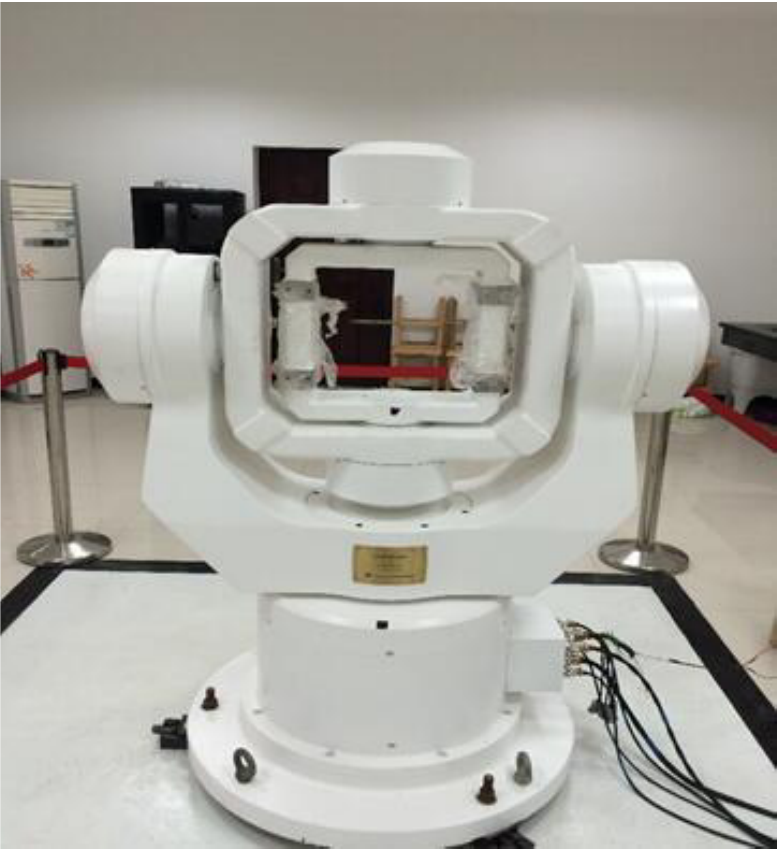
\includegraphics[width=0.34\textwidth]{guide_turntable.png}
\caption{XW-GI7681三轴转台结构}\label{fig:turntable}
\end{figure}
\subsection{IMU初始对准}
使用如图~\ref{fig:100C}所示的中高精度惯性测量单元，
官方型号为NovAtel SPAN IMU-ISA-100C；
其采用光纤陀螺与MEMS加速度计，标称200~Hz输出。
\begin{figure}[htbp]\centering
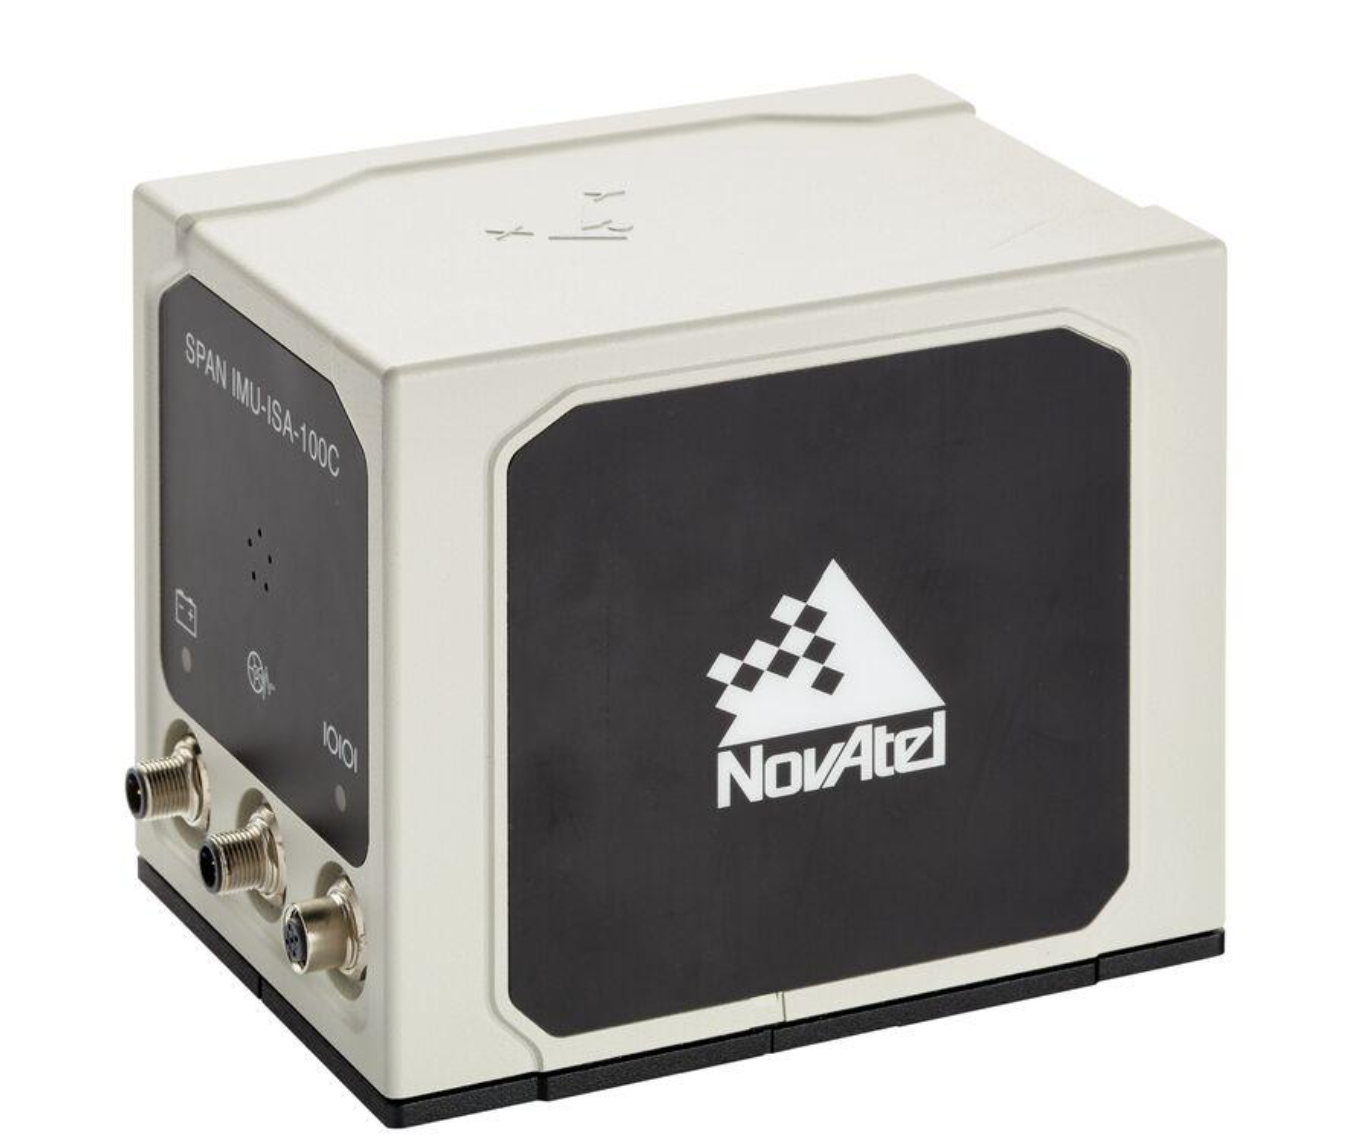
\includegraphics[width=0.43\textwidth]{100C.png}
\caption{NovAtel SPAN IMU-ISA-100C实物图
（来源：NovAtel官方产品页面）}\label{fig:100C}
\end{figure}